% \begin{figure}  % Side caption figure
%     \begin{minipage}{0.62\textwidth}
%     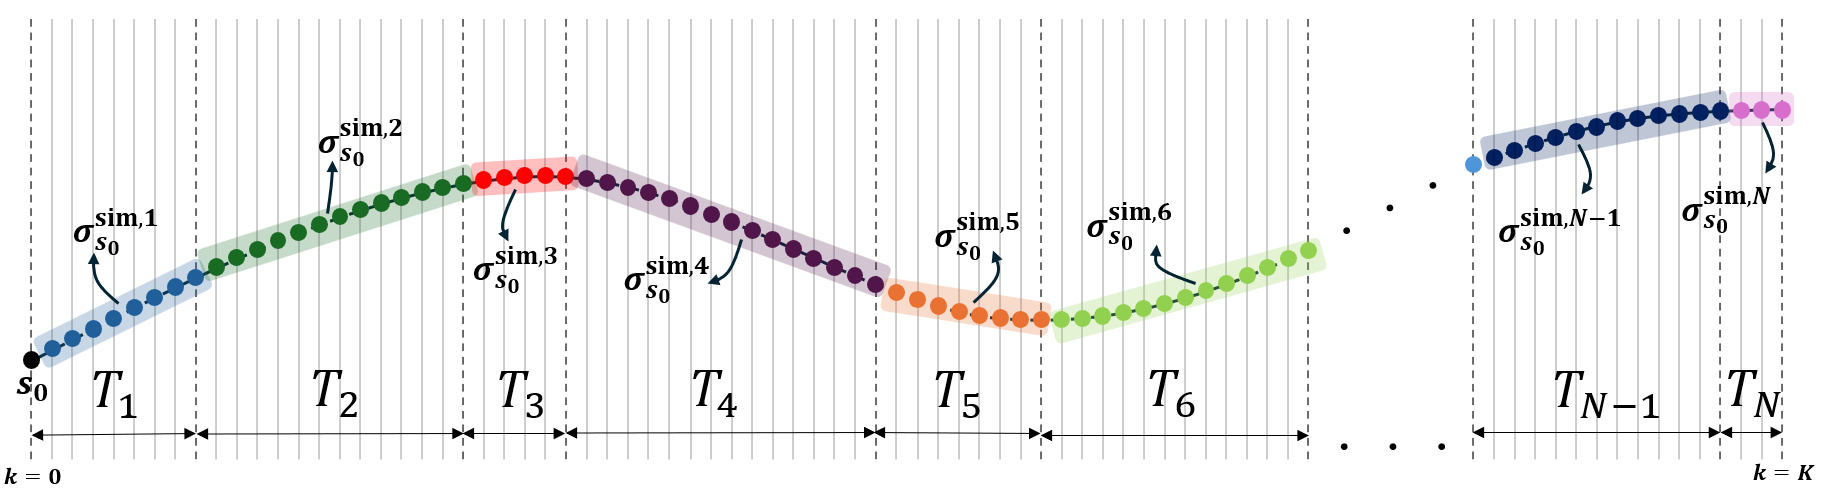
\includegraphics[width=\textwidth]{figures/AAAI_traj2.png} % Replace with your image
%     \end{minipage}
%     \hfill
%     \begin{minipage}{0.35\textwidth}
%     \caption{This figure shows the division of the trajectory into $N$ different segments $\trajsimseg{q}_{\statee_0}, q\in[N]$.}
%     \vspace{-5mm}
%     \label{fig:realization}    
%     \end{minipage}
%     \vspace{-5mm}
% \end{figure}
\begin{figure*}
    \centering
    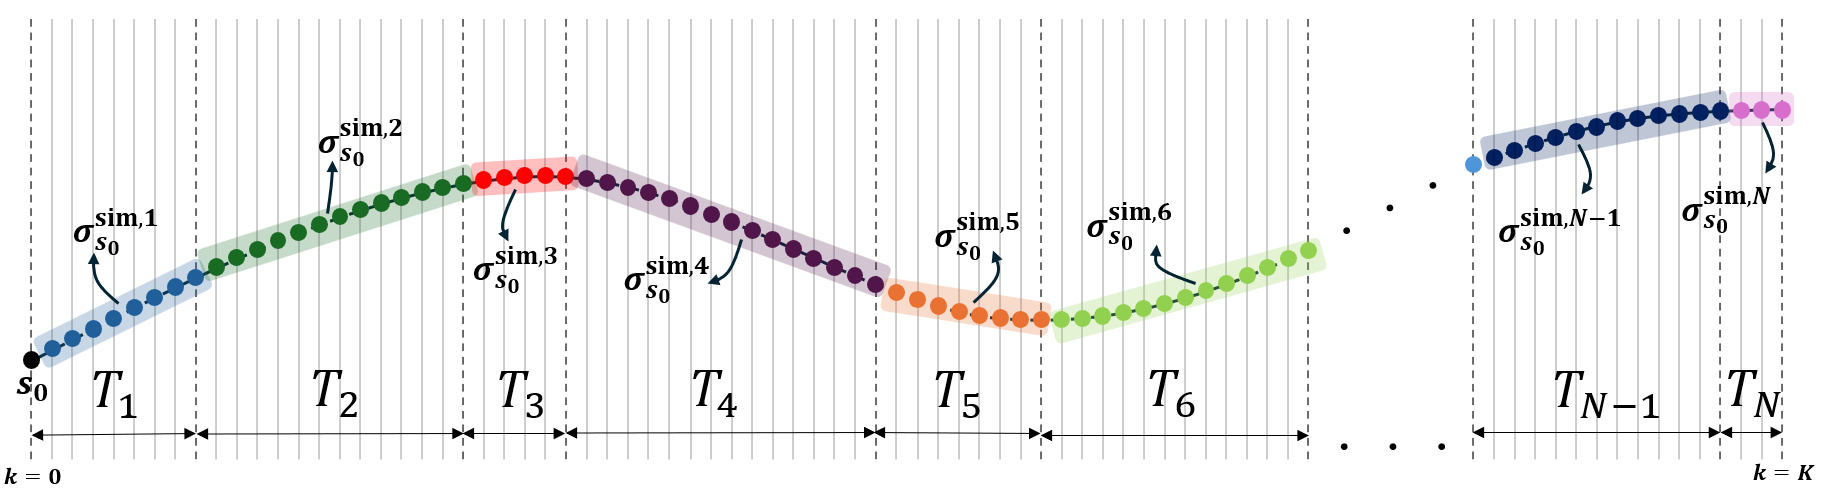
\includegraphics[width = 0.6\textwidth]{figures/AAAI_traj2.png}
    \caption{This figure shows the division of the trajectory into $N$ different segments $\trajsimseg{q}_{\statee_0}, q\in[N]$ }\label{fig:realization}
    \vspace{-5mm}
\end{figure*}

In this section, we introduce a new training strategy for the model $\overallf(\statee_0\ ;\theta)$ that avoids the scalability issues \navid{arising from the surrogate model's large size when handling long time horizons, as encountered in \cite{hashemi2024statistical}}. Figure \ref{fig:realization} illustrates a realization of a trajectory $\trajsim_{\statee_0} :=  \statee_1, \ldots, \statee_{\horizon}$ over the horizon $\horizon$. In this figure, we divide the time horizon into $N$ segments, each with length $T_q$, where $q \in [N]$. We denote each trajectory segment as $\trajsimseg{q}_{\statee_0},\ q \in [N]$, defined as:
\vspace{-3mm}
\begin{equation}
    \trajsimseg{q}_{\statee_0} := \statee_{t_q+1}, \statee_{t_q+2}, \ldots, \statee_{t_q+T_i}, \quad t_q = \sum_{\ell=1}^{q-1} T_\ell,\ t_1 = 0.
\end{equation}
\vspace{-3mm}\\
The key idea is to directly link each trajectory segment $\trajsimseg{q}_{\statee_0},\ q \in [N]$ to its initial state $\statee_0 \in \init$. Thus, we can train an independent model $\overallf_q(\statee_0\ ; \theta_q),\ q \in [N]$ for each segment, which predicts $\trajsimseg{q}_{\statee_0}$ directly based on the initial state $\statee_0$. This model is also used to compute surrogate flowpipes for the trajectory segments $\bar{X}_q, q \in [N]$, representing the image of set $\init$ through the model $\overallf_q(\init\ ; \theta_q)$.

Here are the reasons why this new training strategy for the trajectory $\trajsim_{\statee_0}$ resolves all the scalability issues, we listed for \cite{hashemi2024statistical}, in the Introduction section. \navid{First and foremost,} since all surrogate models $\overallf_q(\statee_0\ ; \theta_q), q \in [N]$ are directly connected to the initial state, we do not need \navid{to iterate} them \navid{sequentially} over the time horizon for prediction of states in  $\trajsimseg{q}_{\statee_0}, q\in[N]$, thus eliminating the problem of cumulative errors over the time horizon. \navid{Furthermore} in this setting, the size of the models $\overallf_q(\statee_0\ ; \theta_q), q \in [N]$ can be small. The small size of the models allows for efficient computation of surrogate flowpipes $\bar{X}_q := \overallf_q(\init\ ; \theta_q)$ for each segment via exact-star reachability analysis\footnote{However, if the set of initial states $\init$ is large and the partitioning of $\init$ is not scalable (high dimensional states), we remain limited to using approx star. Nevertheless, even for this case, the small size of the model significantly reduces the conservatism of approx star.}. 
\navid{Additionally, } the smaller models $\overallf_q(\statee_0\ ; \theta_q), q \in [N]$ enable efficient training of accurate models for each trajectory segment. \navidg{Furthermore, although we have to train more models using this technique,  we can train them in parallel as they are totally independent processes.}
% \item It eliminates the constraints identified in \cite{hashemi2024statistical} for performing reachability analysis over long horizon, making it a better option for real-world applications.
% \item The smaller size of the models $\overallf_q(\statee_0\ ; \theta_q), q \in [N]$ also enables efficient training of accurate models for each segment of the trajectory.

\navid{Once the surrogate flowpipes \( \bar{X}_q = \langle \bar{c}_q, \bar{V}^q, \bar{P}_q \rangle \), for \( q \in [N] \), are obtained as star sets, the surrogate flowpipe for the entire trajectory forms another star set, \( \bar{X} = \langle \bar{c}, \bar{V}, \bar{P} \rangle \). This global surrogate flowpipe is constructed by concatenating all individual star sets \( \bar{X}_q \), for \( q \in [N] \), which implies: $\bar{c} = \left[ \bar{c}_1^\top , \ldots , \bar{c}_N^\top \right]^{\top}$, $\bar{V} = \mathbf{diag}\left(\bar{V}^1, \ldots, \bar{V}^N\right)$ and $\bar{P} = \bigwedge_{q=1}^N \bar{P}_q.$  }
% \navid{Once the surrogate flowpipes $\bar{X}_q = \langle \bar{c}_q, \bar{V}^q, \bar{P}_q \rangle  , q \in [N]$ are obtained as star sets}, we can concatenate them to provide a single star-set as the surrogate flowpipe for the entire trajectory. We later inflate this set with the inflating hypercube to obtain the $\delta$-confident flowpipe. 

% In this section, we provide a new setting for training the model, $\overallf(\statee_0\ ;\theta)$ that does not face the scalability issues listed for \cite{hashemi2023data, hashemi2024statistical}. Fig.\ref{fig:realization} shows a realization of a trajectory $\trajsim_{\statee_0} := \statee_0, \statee_1, \cdots, \statee_{\horizon}$ over the horizon $\horizon$. In this figure, we segment the time horizon into $N$ different segmentations with length $T_i , i \in[N]$. We also denote each trajectory partition as $\trajsimseg{i},\ i\in[N]$, where,
% \[
% \trajsimseg{i}_{\statee_0} := \statee_{t+1},\ \statee_{t+2},\ \cdots,\ \statee_{t+T_i},\quad t = \sum_{\ell=1}^{i-1} T_\ell.
% \]
% The main idea is to directly connect every trajectory partition $\trajsimseg{i}_{\statee_0},\ i \in [N]$ to its initial state $\statee_0 \in \init$. In other words, we train a completely independent model $\overallf_i(\statee_0\  ; \theta_i) , i\in[N]$ for each segment such that it predicts $\trajsimseg{i}_{\statee_0}$ directly based on the initial state $\statee_0$. We also utilize this model to compute the surrogate flowpipes for the trajectory partitions $\bar{X}_i, i\in[n]$ which are the image of set $\init$ through the model $\overallf_i(\init\ ;\theta_i)$. 

% Here, we provide reasoning for why this new setting for training the trajectory $\trajsim_{\statee_0}$ resolves for all the scalability issues listed for \cite{hashemi2023data, hashemi2024statistical}.
% \begin{enumerate}[wide, labelwidth=!, labelindent=0pt]
% \item Since all the surrogate models $\overallf_i(\statee_0\ ;\theta_i) , i\in[N]$ are directly connected to the initial state, we are not required to unroll them over the time horizon. This implies we do not face the problem of cumulative errors over the time horizon.
% \item Since we train a different model for every partition $i \in [N]$ of the trajectory, our model can also predict the periodic behavior of the trace.
% \item Since the models $\overallf_i(\statee_0\ ;\theta_i), i\in [n]$ are relatively small, and they are directly connected to the initial state $\statee_0 \in \init$. The surrogate flowpipe $\bar{X}_i := \overallf_i(\init\ ;\theta_i)$, for every partition $i \in [N]$, can be computed efficiently via exact-star reachability analysis.
% \item Since the models $\overallf_i(\statee_0\ ;\theta_i), i\in [n]$ are relatively small, we can efficiently train an accurate model for every partition $i\in [N]$.

% \end{enumerate}
